\documentclass[11pt]{article}
\usepackage[margin=1in]{geometry}
\usepackage{amsmath,amssymb}
\usepackage{booktabs}
\usepackage{siunitx}
\usepackage{graphicx}
\usepackage{float}
\usepackage{hyperref}

\title{GridFM Data Generation Methodology and Formulation \\
IEEE RTS 24-Bus with Droop Control (10,000 Scenarios)}
\author{}
\date{\today}

\begin{document}
\maketitle

\section{Objective}
This document describes the exact formulation, data-generation workflow, and validation results used to produce the dataset:
\begin{center}
\texttt{graphkit\_data/case24\_ieee\_rts\_s10000\_droop\_mprange\_mqrange}
\end{center}
for subsequent training in GridFM-GraphKit.

\section{Case Configuration Used}
The run used IEEE RTS 24-bus power flow (PF) with droop control enabled and randomized droop gains.

\begin{table}[H]
\centering
\caption{Generation settings used in GridFM DataKit}
\begin{tabular}{ll}
\toprule
Item & Value \\
\midrule
Network case & \texttt{case24\_ieee\_rts} \\
Scenarios & 10,000 \\
Buses & 24 \\
Mode & PF \\
Droop enabled & Yes \\
Reference bus & bus 1 \\
$V_0$ & 1.1 p.u. \\
Voltage limits & $V_{\max}=1.2$ p.u. (all buses), $V_{\min}=0.95$ p.u. \\
Droop buses & 11 buses: 1,2,7,13,14,15,16,18,21,22,23 \\
$m_p$ range & $[0.03, 0.05]$ \\
$m_q$ range & $[0.02, 0.04]$ \\
Frequency deadband & 0.006 \\
Voltage deadband & 0.001 \\
Load scaling & fixed at 1.0 (no random load scaling) \\
\bottomrule
\end{tabular}
\end{table}

\section{Power-Flow and Droop Formulation}
\subsection{AC Power Balance}
For each bus $i$, active and reactive balance equations are solved in polar form:
\begin{align}
P_i &= V_i \sum_{j=1}^{N} V_j \left(G_{ij}\cos(\theta_i-\theta_j) + B_{ij}\sin(\theta_i-\theta_j)\right), \\
Q_i &= V_i \sum_{j=1}^{N} V_j \left(G_{ij}\sin(\theta_i-\theta_j) - B_{ij}\cos(\theta_i-\theta_j)\right).
\end{align}
Here $G_{ij}$ and $B_{ij}$ come from the admittance matrix used by the case.

\subsection{Droop Control Law}
Droop control is applied on configured droop buses. Conceptually:
\begin{align}
\Delta f &= f - f_0, \\
\Delta V &= V - V_0,
\end{align}
and active/reactive power adjustments follow droop slopes:
\begin{align}
\Delta P &\propto -\frac{1}{m_p} \Delta f, \\
\Delta Q &\propto -\frac{1}{m_q} \Delta V,
\end{align}
with deadband behavior around nominal values (frequency deadband 0.006, voltage deadband 0.001). In the exported node data, each bus includes:
\begin{center}
\texttt{mp\_droop, mq\_droop, frequency\_deadband, voltage\_deadband}
\end{center}
Non-droop buses are encoded with \texttt{mp\_droop=0} and \texttt{mq\_droop=0}.

\subsection{Operational Limits}
The PF solution is constrained by case limits, most critically voltage bounds:
\begin{align}
V_i^{\min} \le V_i \le V_i^{\max}, \quad \forall i,
\end{align}
with $V_i^{\max}=1.2$ p.u. used to avoid feasibility collapse under droop updates.

\section{Dataset Construction Methodology}
\subsection{Raw Solver Outputs}
GridFM generated raw per-scenario outputs under:
\begin{center}
\texttt{data\_out\_case24\_s10000\_droop\_mprange\_mqrange/case24\_ieee\_rts/raw}
\end{center}
including bus, branch/admittance, generator, and runtime logs.

\subsection{GraphKit Projection}
Raw outputs were projected to GraphKit-ready files:
\begin{itemize}
\item Node file: \texttt{raw/pf\_node.csv}
\item Edge file: \texttt{raw/pf\_edge.csv}
\end{itemize}

Node columns:
\begin{center}
\texttt{scenario, bus, Pd, Qd, Pg, Qg, Vm, Va, PQ, PV, REF,} \\
\texttt{mp\_droop, mq\_droop, frequency\_deadband, voltage\_deadband}
\end{center}

Edge columns:
\begin{center}
\texttt{scenario, index1, index2, G, B}
\end{center}

\subsection{Scenario Split}
Fixed split used for ML reproducibility:
\begin{itemize}
\item Train: scenarios 0--7999 (8,000)
\item Validation: scenarios 8000--8999 (1,000)
\item Test: scenarios 9000--9999 (1,000)
\end{itemize}

\section{Measured Results (from this run)}
\subsection{Core counts}
\begin{table}[H]
\centering
\caption{Dataset cardinalities}
\begin{tabular}{lr}
\toprule
Metric & Value \\
\midrule
Total scenarios & 10,000 \\
Buses per scenario & 24 \\
Node rows & 240,000 \\
Edge rows & 920,000 \\
Droop-enabled bus rows & 110,000 \\
\bottomrule
\end{tabular}
\end{table}

\subsection{Electrical output statistics}
\begin{table}[H]
\centering
\caption{Selected PF output statistics (all node rows)}
\begin{tabular}{lrrrr}
\toprule
Variable & Mean & Std & Min & Max \\
\midrule
$V_m$ (p.u.) & 1.09097 & 0.02150 & 1.05159 & 1.16493 \\
$V_a$ (deg) & 6.63103 & 8.91438 & -5.71074 & 24.43158 \\
$m_p$ & -- & -- & 0.00000 & 0.05000 \\
$m_q$ & -- & -- & 0.00000 & 0.04000 \\
\bottomrule
\end{tabular}
\end{table}

\subsection{Runtime and frequency-deviation statistics}
\begin{table}[H]
\centering
\caption{Per-scenario runtime and frequency deviation}
\begin{tabular}{lrrrr}
\toprule
Variable & Mean & Std & Min & Max \\
\midrule
AC runtime (s) & 0.20398 & 0.03540 & 0.08900 & 0.51100 \\
Frequency deviation & -1.6799\times10^{-4} & 2.4215\times10^{-5} & -2.5217\times10^{-4} & -1.1435\times10^{-4} \\
\bottomrule
\end{tabular}
\end{table}

\section{Figures}
\begin{figure}[H]
\centering
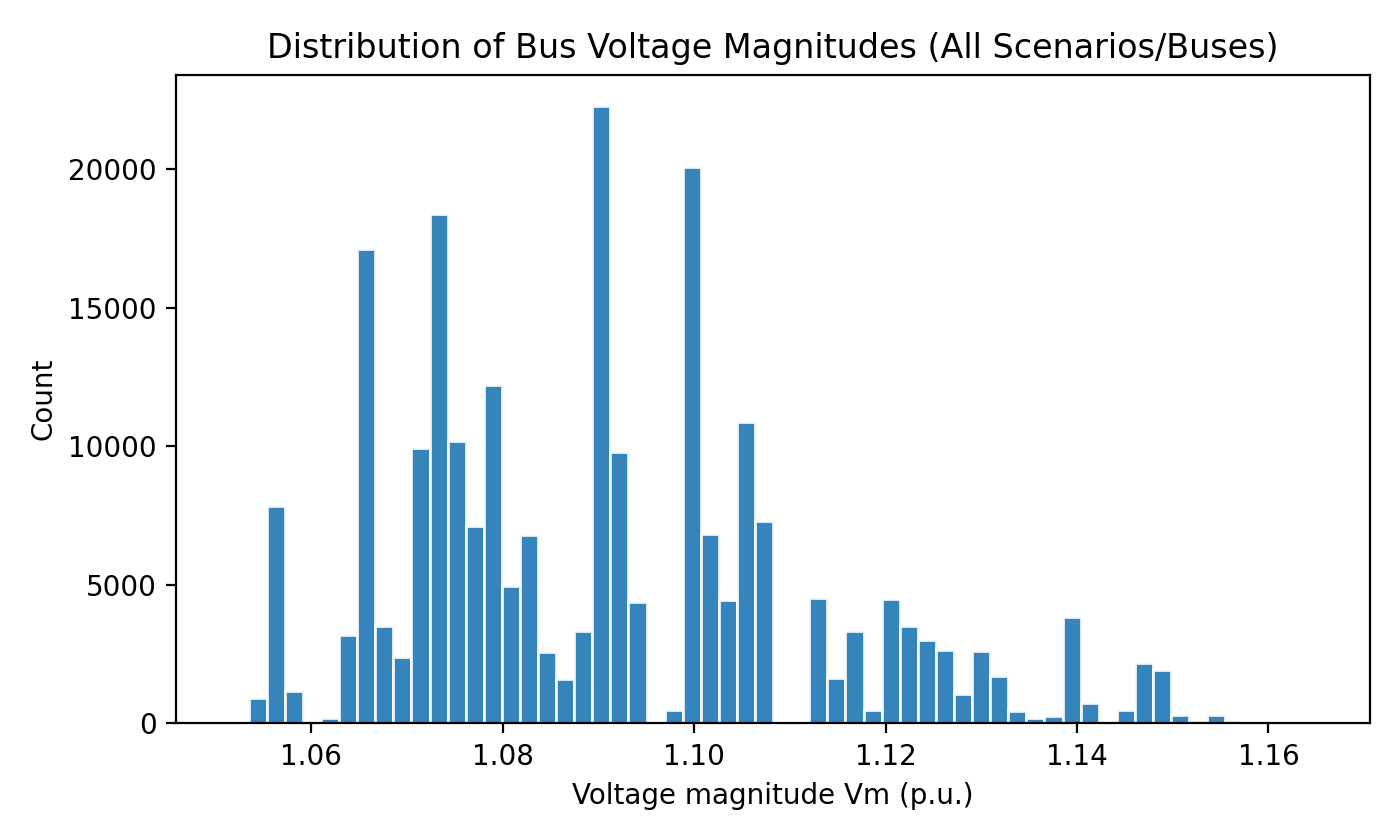
\includegraphics[width=0.8\linewidth]{fig_vm_distribution.png}
\caption{Distribution of voltage magnitudes across all buses and scenarios.}
\label{fig:vm_dist}
\end{figure}

\begin{figure}[H]
\centering
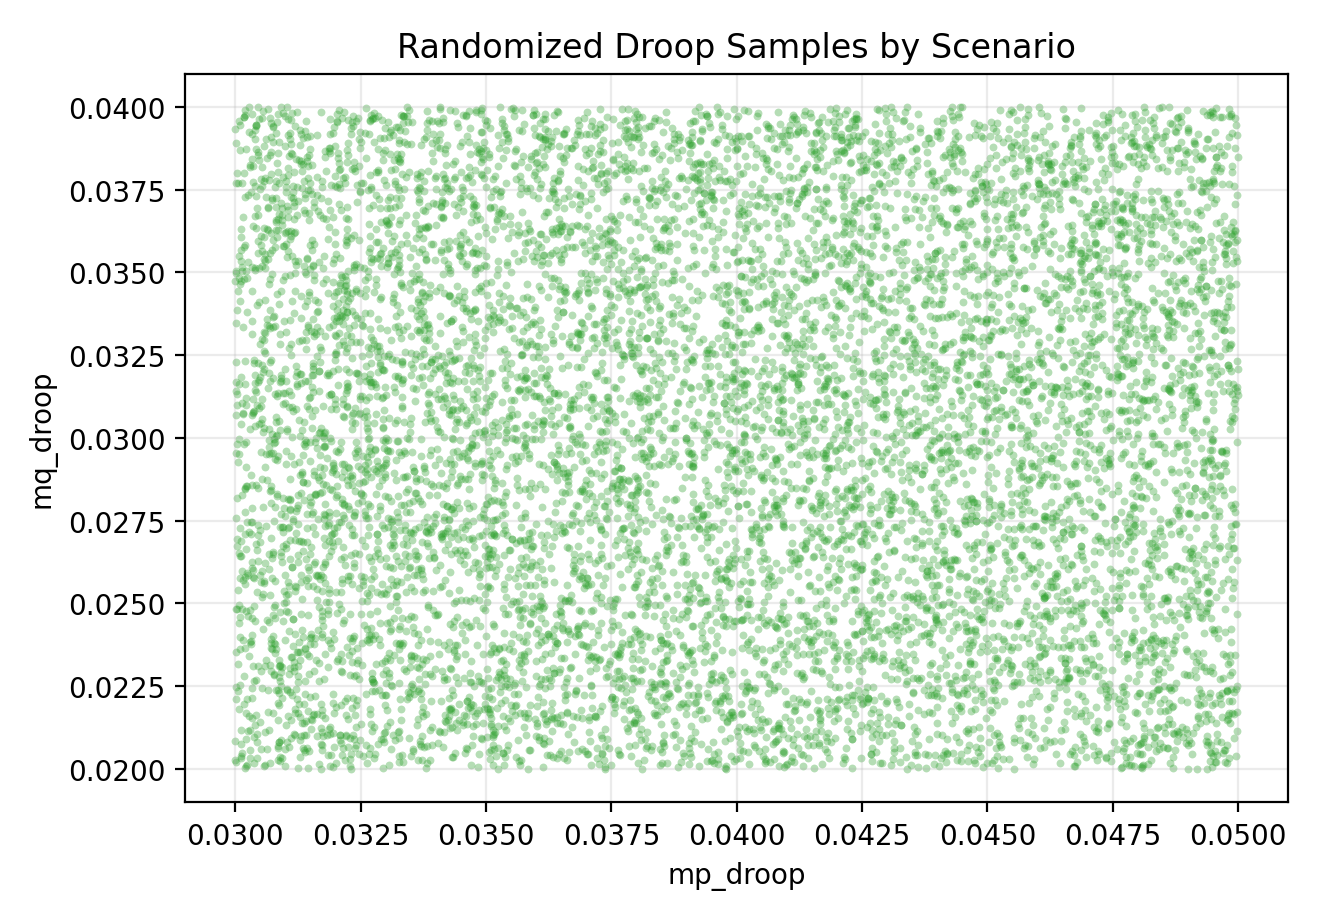
\includegraphics[width=0.75\linewidth]{fig_droop_parameter_scatter.png}
\caption{Randomized droop gain samples by scenario ($m_p$ vs $m_q$).}
\label{fig:droop_scatter}
\end{figure}

\begin{figure}[H]
\centering
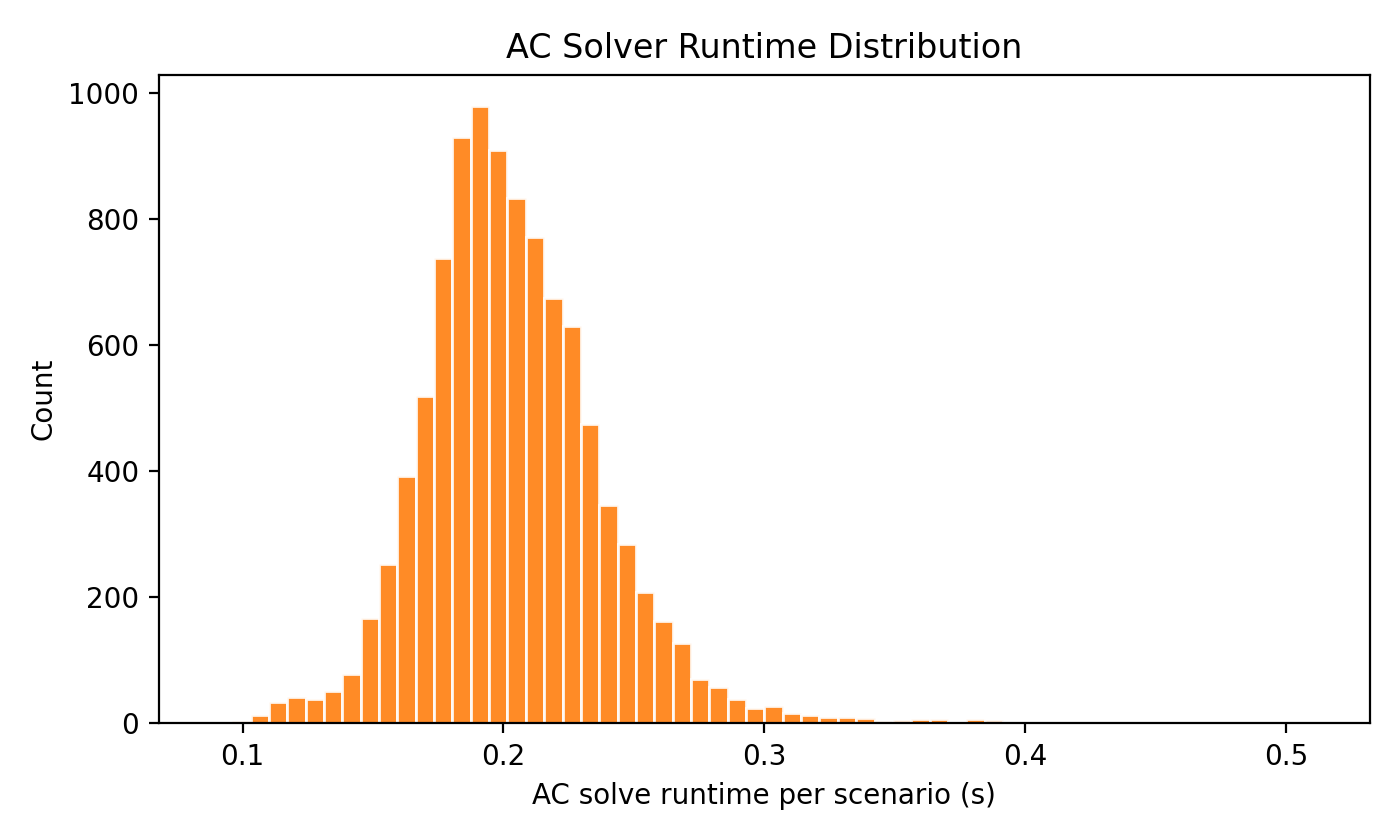
\includegraphics[width=0.8\linewidth]{fig_ac_runtime_distribution.png}
\caption{Distribution of per-scenario AC solve runtime.}
\label{fig:runtime_dist}
\end{figure}

\begin{figure}[H]
\centering
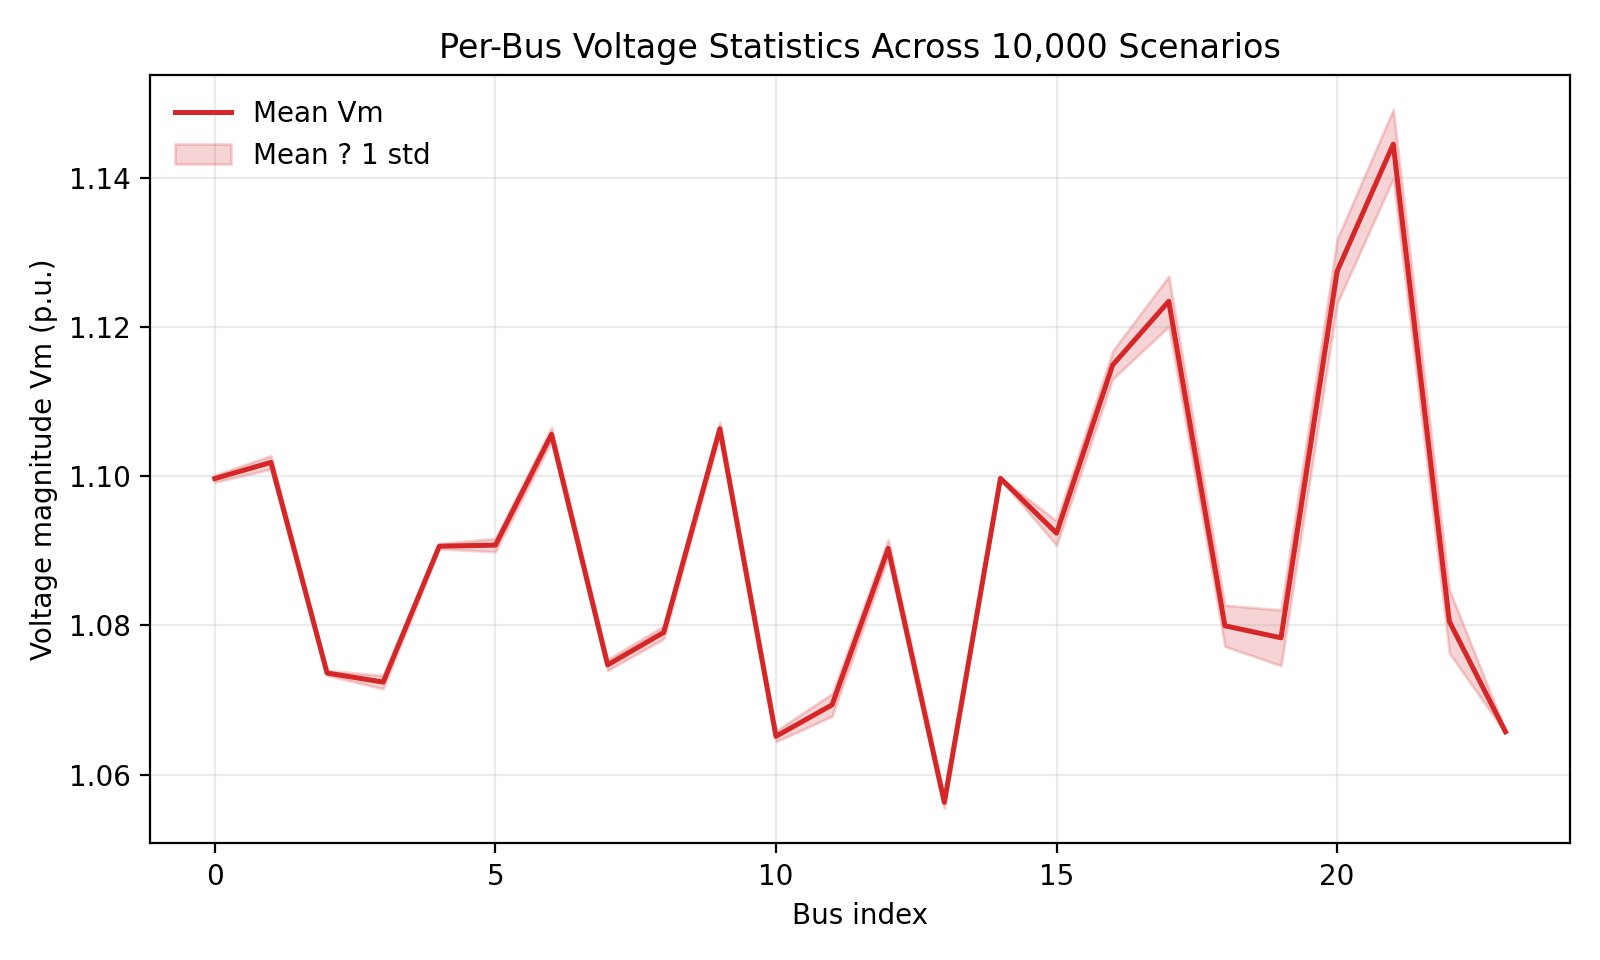
\includegraphics[width=0.85\linewidth]{fig_vm_by_bus_mean_std.png}
\caption{Per-bus voltage mean and $\pm1\sigma$ envelope over 10,000 scenarios.}
\label{fig:vm_bus}
\end{figure}

\section{Discussion}
\begin{itemize}
\item The generated dataset is large enough for GNN training (240k node samples, 920k edge samples) and preserves control-relevant inputs through explicit droop/deadband features.
\item Voltage magnitudes remain within configured limits for all exported points (observed range: 1.0516--1.1649 p.u.), indicating stable operation under this parameterization.
\item Runtime distribution is narrow (mean 0.204 s/scenario), so regeneration and ablation sweeps are practical.
\item Because load scaling was fixed at 1.0, scenario diversity comes mainly from droop randomization. If higher diversity is needed for ML generalization, vary load/generation perturbations in future runs.
\end{itemize}

\section{Files to Transfer to GridFM-GraphKit}
Copy this folder as-is:
\begin{center}
\texttt{graphkit\_data/case24\_ieee\_rts\_s10000\_droop\_mprange\_mqrange}
\end{center}
Key files are \texttt{raw/pf\_node.csv}, \texttt{raw/pf\_edge.csv}, and \texttt{scenario\_split.json}.

\end{document}
